\documentclass[11pt]{article}
%%%%%%%%%%%% PREAMBULO %%%%%%%%%%%%%%%%%%
\usepackage[T1]{fontenc}%indica que usamos la ñ
\usepackage[utf8]{inputenc}%indica el tipo de codificación ISO-8859-1 (latin)ó utf8
\usepackage[spanish]{babel}%indica que escribiremos en español
\title{plantilla para reportes mecatrónica-mecánica UTA}
\usepackage{amsmath}
\usepackage{amssymb,amsfonts,latexsym}
\usepackage{graphicx}
\usepackage{epstopdf}%para convertir figuras a formato pdf
\usepackage{color}
\usepackage{url}  \urlstyle{same}%para conectar url strings en bibliografías
\usepackage{enumitem}
\usepackage{subfigure}%para colocar varias figuras
\usepackage{multicol}
\usepackage{changepage}
\usepackage{float}%para colocar las tablas como H
\usepackage{array}%dar formato a las tablas
\usepackage{longtable}%dar formato a las tablas
\usepackage{bm}
\usepackage{capt-of}
\usepackage{sidecap}
\usepackage[table,xcdraw]{xcolor}
\sidecaptionvpos{figure}{c}
\usepackage{caption}
\usepackage{commath}
\usepackage{cancel}
\usepackage{lipsum}
%%%%%%%%%%% CONFIGURACION DEL DOCUMENTO %%%%%%%%%%%%%
\usepackage{anysize}%para personalizar el ancho de los margenes
\marginsize{2cm}{2cm}{2cm}{2cm}%izquierda, derecha, arriba, abajo
\usepackage{anyfontsize}

% Para que las referencias sean hipervínculos a las figuras o ecuaciones y
% aparezcan en color
\usepackage[colorlinks=true,plainpages=true,citecolor=blue,linkcolor=blue]{hyperref}
%\usepackage{hyperref} 
% Para agregar encabezado y pie de página
\usepackage{fancyhdr} 
\pagestyle{fancy}
\fancyhf{}
\fancyhead[L]{\footnotesize FICH} %encabezado izquierda
\fancyhead[R]{\footnotesize Centis Mateo}   % dereecha
\fancyfoot[R]{\footnotesize Entregable 3}  % Pie derecha
\fancyfoot[C]{\thepage}  % centro
\fancyfoot[L]{\footnotesize Ingeniería en informática}  %izquierda
\renewcommand{\footrulewidth}{0.4pt}
\usepackage{listings} % Para usar código fuente

% configuración para el lenguaje que queramos utilizar
\definecolor{mygreen}{rgb}{0,0.6,0}
\definecolor{mygray}{rgb}{0.5,0.5,0.5}
\definecolor{mymauve}{rgb}{0.58,0,0.82}
\definecolor{myorange}{rgb}{0.855,0.576,0.027}
\definecolor{backcolour}{rgb}{0.95,0.95,0.92}
\lstset{
language=Octave,
frame=single,   
morecomment = [l][\itshape\color{mygreen}]{\%},
keywordstyle=\color{blue},
commentstyle=\color{mygreen},	
breakatwhitespace=false,         
breaklines=true,  
%numbers=left,
%numbersep=5pt,
basicstyle=\linespread{0.9}\ttfamily\small,
%numberstyle=\tiny\color{mygray}, 
showstringspaces=false, 
showtabs=false,                  
tabsize=2,
stringstyle=\color{myorange},
title=\lstname,
literate=
{+}{{{\color{red}+}}}1
{-}{{{\color{red}-}}}1
{*}{{{\color{red}*}}}1
{,}{{{\color{red},}}}1
{=}{{{\color{red}=}}}1
{)}{{{\color{red})}}}1
{(}{{{\color{red}(}}}1 
{;}{{{\color{red};}}}1
{:}{{{\color{red}:}}}1
{[}{{{\color{red}[}}}1
{]}{{{\color{red}]}}}1
{>}{{{\color{red}>}}}1
}
\title{Plantilla para informes ing. mecanica-mecatronica}

%%%%%%%%%%% COMIENZO DEL DOCUMENTO %%%%%%%%%%%%
\begin{document}

%%%%%%%%%%%%%%%%%%%%%%%%%%%%%%%%%% PORTADA %%%%%%%%%%%%%%%%%%%%%%%%%%%%%%%%%%%%%%%%%%%%

\begin{center}																		%%%
	\newcommand{\HRule}{\rule{\linewidth}{0.5mm}}									%%%\left

	%%%

	%%%
	\vspace*{1.0cm}								%%%
	%%%	
	\textsc{\huge UNL - FICH \vspace{5px}}\\[1.5cm]

	\textsc{\LARGE Cálculo numérico - Entregable 3}\\[1.5cm]													%%%

	\textsc{\LARGE Centis Mateo}

\end{center}

%%%%%%%%%%% CUERPO DEL DOCUMENTO
\section*{Enunciado}
La trayectoria de una partícula que inicialmente se encuentra en el punto
$(-1, 1)$ y se mueve en el plano está dada por la curva $(x_1(t), x_2(t))$, donde las funciones x1 y x2 son la solución del siguiente sistema de ecuaciones diferenciales:
\begin{equation*}
	\left\{
	\begin{array}{ll}
		x'_1(t)=-tx_2(t), \\
		x'_2(t)=tx_1(t)-tx_2(t)
	\end{array}
	\right.
\end{equation*}

\begin{enumerate}[label=(\alph*)]
	\item Grafique la trayectoria de la partícula durante los primeros 20 segundos.
	\item Utilice el método de Runge-Kutta 4 con paso h = 0.1 para determinar la posición de la
	      partícula y su rapidez a los tres segundos.
	\item ¿Cuántos dígitos correctos tienen los resultados del item anterior? Explique cómo lo determinó.
	\item Recuerde que la longitud de la trayectoria de la partícula durante los T primeros segundos
	      está dada por $\int_0^T\sqrt{x'_1(t)^2+x'_2(t)^2}dt$.
	      \begin{enumerate}[label=(\roman*)]
		      \item Realice interpolación de $x_1(t)$ y de $x_2(t)$ con los datos obtenidos en (b), por medio
		            de spline cúbico sujeto. Explique cómo obtiene las condiciones de las derivadas en los
		            extremos.
		      \item Utilice la interpolación realizada anteriormente para estimar la distancia recorrida por
		            la partícula durante los primeros tres segundos.
	      \end{enumerate}
	\item Determine el instante de tiempo a partir del cual la partícula está siempre a una distancia
	      menor a 0.01 del origen de coordenadas.
\end{enumerate}

\newpage

\section*{Resolución}
A fin de llevar a cabo la resolución del enunciado, se comenzó definiendo en Octave el sistema de ecuaciones diferenciales de primer orden como una función vectorial.

\subsection*{a.}

Para graficar la trayectoria de la partícula durante los primeros 20 segundos, se utilizó el método de \textit{Runge-Kutta} de orden 4 para obtener las soluciones del sistema. Aunque Runge-Kutta requiera de 4 evaluaciones de la función por cada paso contra 1 del método de \textit{Euler}, su convergencia es superior al método de Euler, es decir, con pequeños cambios en el h elegido se pudo observar como la aproximación era prácticamente igual a la solución real. En cambio, utilizando el método de Euler es necesario un h muy chico para que la aproximación sea "buena".

Por lo tanto, para realizar la gráfica se definió como punto inicial de la partícula $y_0=(-1,1)$ y como intervalo de tiempo $[0,20]$. Por consiguiente, se tomó un tamaño del intervalo $h=0.01$, dado este valor podemos calcular el número de intervalos que se da como $n=\frac{b-a}{h}$, dando un total de $n=\frac{20-0}{0.025}=800$ intervalos. Con estos datos se llamó al método anteriormente mencionado y se obtuvieron los vectores solución del sistema de ecuaciones diferenciales $x_1(t)$ y $x_2(t)$.

Con estos vectores, se procedió a realizar la gráfica $x_1(t)$ vs $x_2(t)$ para los primeros 20 segundos.
\\
\setkeys{Gin}{width=1.0\textwidth}
\begin{figure}[h]
	\centering
	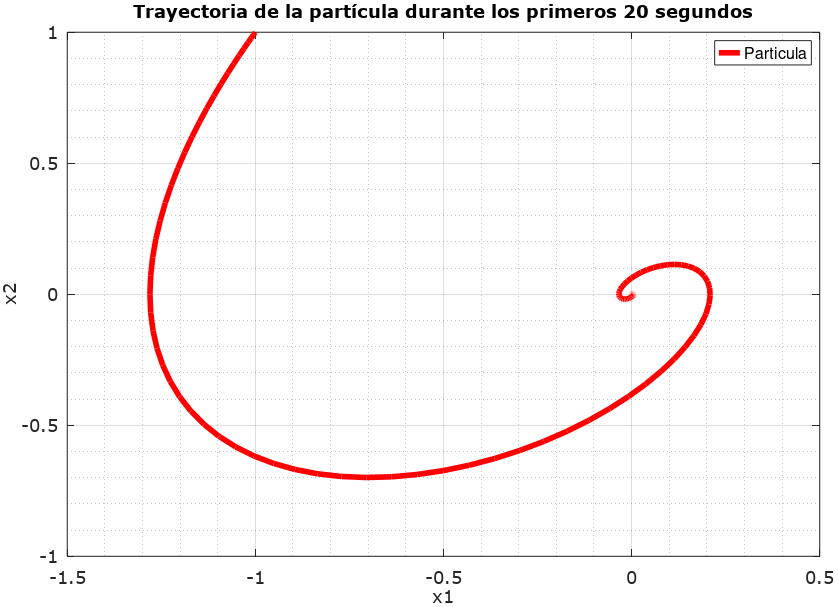
\includegraphics{trayectoria20s3.png}
\end{figure}

\subsection*{b.}

Para determinar la posición y la rapidez de la partícula a los 3 segundos se usó de nuevo el método de Runge-Kutta de orden 4. En este caso, se pasó un intervalo $[0,3]$ para facilitar la búsqueda del momento $t=3s$ y un paso $h=0.1$.

A través de los vectores solución $x_1(t)$ y $x_2(t)$ se obtuvo la posición en tiempo $t=3s$ accediendo a su posición final. Luego, para obtener la rapidez de la partícula, se hizo uso del sistema de ecuaciones diferenciales para obtener los valores de las derivadas $x'_1(t)$ y $x'_2(t)$ en el momento $t=3s$ reemplazando $t=3$, y a estas se le aplicó la función \textit{norm} para obtener la rapidez:

\begin{equation*}
	\begin{split}
		x'_1(3)=-0.14541, x'_2(3)=0.46032\\
		norm([-0.14541,0.46032])=0.48273
	\end{split}
\end{equation*}

Se procedió a graficar la posición de la partícula a los 3 segundos.
\begin{figure}[h]
	\centering
	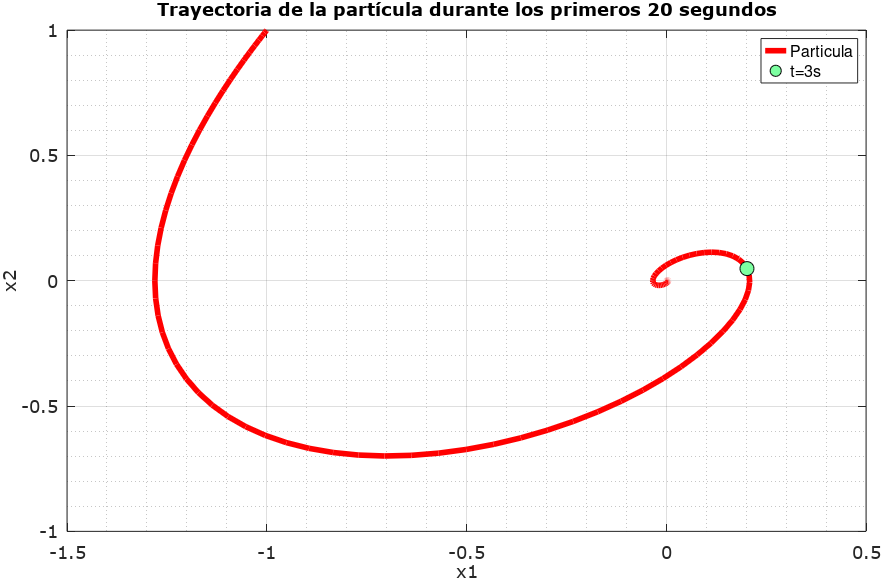
\includegraphics{trayectoria20s2.png}
\end{figure}\\

\subsection*{c.}
Para resolver el inciso (c) se fue observando la cantidad de cifras significativas en común en los resultados del inciso (b) para diferentes número de pasos. De esta manera se fue duplicando la cantidad de pasos.

Observando la tabla, se puede concluir como duplicando el número de pasos, se van ganando cifras significativas progresivamente según el orden del método.

\begin{table}[h]
	\centering
	\begin{tabular}{|c|c|c|c|}
		\hline
		\rowcolor[HTML]{38FFF8}
		\textbf{n}   & \textbf{posición X} & \textbf{posición Y} & \textbf{módulo rapidez} \\ \hline
		\textbf{15}  & 0.2022834091442048  & 0.04877480732237864 & 0.4832130523523182      \\ \hline
		\textbf{30}  & 0.2019150006882205  & 0.04847275127510394 & 0.48274960765413        \\ \hline
		\textbf{60}  & 0.2018961295582949  & 0.04845318566594918 & 0.4827339164423362      \\ \hline
		\textbf{120} & 0.2018950846066559  & 0.0484519675978198  & 0.4827333113566826      \\ \hline
	\end{tabular}
\end{table}

Se observa comparando la solución para 30 pasos con la de 60 pasos, obteniendo de la diferencia de estas el error absoluto $error_{abs}=|sol30-sol60|=1.569121179378907e-05$, por lo tanto la solución del inciso (b) tiene 4 dígitos correctos.

\subsection*{d.}

Se utilizó la función \textit{funcion$\_$spline}, que recibe como parámetros el vector t y la solución $x_i(t)$ correspondiente, y se encarga de armar la función spline $S(x)$ y su derivada $dS(x)$, esta hace uso de la función \textit{Spline$\_$Cubico$\_$Sujeto} para obtener los coeficientes de la interpolación. Por lo que se necesitan los valores de la derivada en cada extremo del intervalo, estos valores son obtenidos de las derivadas del inciso (b). También sería posible usar un método e derivación numérica pero este posee una precisión menor y no estaríamos aprovechando la información sobre la forma de la derivada que tenemos.

\begin{figure}[h]
	\centering
	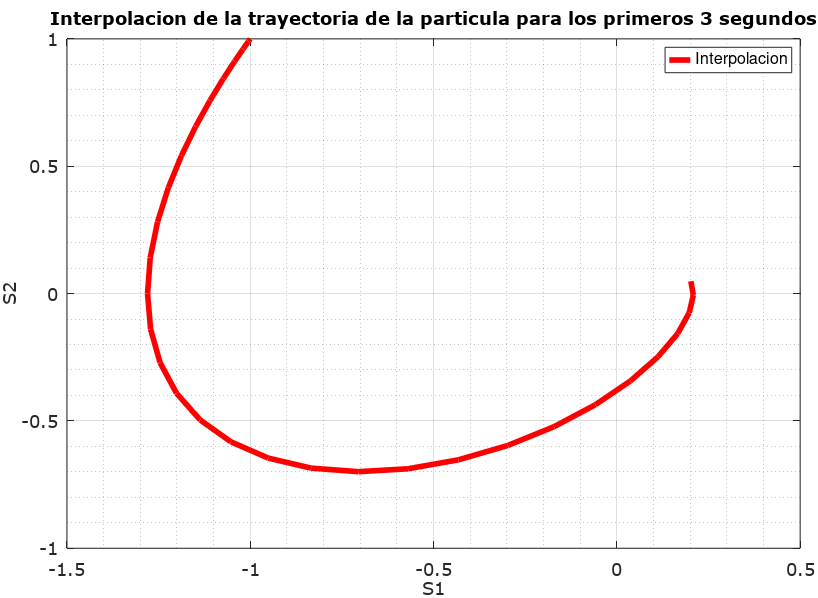
\includegraphics{interpolacion.png}
\end{figure}

Haciendo uso de lo anterior mencionado, se logró estimar que la distancia recorrida por la partícula durante los primeros tres segundo fue de $\int_0^3\sqrt{x'_1(t)^2+x'_2(t)^2}dt=3.3543$.

%inciso (d)
\subsection*{d.}
Para encontrar el instante de tiempo para el cual la partícula está siempre a una distancia menor qu e 0.01 se armó de forma similar al inciso anterior, una spline que interpola los puntos solución para cada uno de los vectores solución del sistema de ecuaciones diferenciales. Con estas funciones se armó la función distancia: $d(x)=\sqrt{(S1(x)-x_2)^2+(S2(x)-y_2)^2}$, como queremos encontrar la distancia al origen $(x_2,y_2)=(0,0)$, la función se convierte en $d(x)=\sqrt{S1(x)^2+S2(x)^2}$.

Se halló el instante de tiempo iterando sobre el vector de tiempo, evaluando en cada iteración que la distancia evaluada en el i-ésimo tiempo hasta encontrar el tiempo para el cual la distancia sea menor al valor deseado 0.01.

De esta manera se encontró que el valor de tiempo para el cual la distancia siempre es menor a 0.01 es $tiempoMenor=4.6s$.
\clearpage
\begin{center}
	\newcommand{\HRule}{\rule{\linewidth}{0.5mm}}
	\vspace*{1.0cm}								%%%
	%%%	
	\textsc{\huge \underline{ANEXO} \vspace{5px}}\\

\end{center}
\begin{lstlisting}[caption=Entregable3.m]
	%Ejercicio Entregable 3
	f=@(t,x)[-t*x(2);%x(1) y x(2) son las "incognitas" del sistema.
			 t*x(1)-t*x(2)];
	%----------------------------------------------------------------------------------------------
	%a)Grafico de la trayectoria de la particula durante los primeros 20 segundos
	%grafico x1 vs x2
	y0=[-1;1];
	a=0;
	b=20;
	h=0.05;
	n=(b-a)/h+1;
	[t,xRes]=rungeKutta4(f,a,b,y0,n);
	fig1= figure(1);
	plot(xRes(:,1),xRes(:,2),'r-','linewidth',4);
	FN = findall(fig1,'-property','FontName');
	title('Trayectoria de la particula durante los primeros 20 segundos')
	xlabel('x1');
	ylabel('x2');
	grid on 
	grid minor on
	set(FN,'FontName','C:\Users\Mateo\AppData\Local\Microsoft\Windows\Fonts\DankMono-Regular.ttf');
	FS = findall(fig1,'-property','FontSize');
	set(FS,'FontSize',18);
	hold on
	
	%---------------------------------------------------------------------------------------------
	%b)Utilizar metodo de RungeKutta4 con paso h=0.1 para determinar 
	%su posicion y velocidad a los 3 segundos.
	hRK=0.1;
	aRK=0;
	bRK=3;
	nRK=(bRK-aRK)/hRK+1;
	[tRK xRK]=rungeKutta4(f,aRK,bRK,y0,nRK);
	x1RK=xRK(:,1);%x1(t) Posicion en X en el tiempo (t)
	x2RK=xRK(:,2);%x2(t) Posicion en Y en el tiempo (t)
	%posicion en tiempo t=3s
	posX=x1RK(length(x1RK));
	posY=x2RK(length(x2RK));
	%rapidez en tiempo t=3s
	dx1RK=-3*posY;
	dx2RK=3*posX-3*posY;
	modRap=norm([dx1RK,dx2RK]);
	plot(posX,posY,'o','MarkerEdgeColor','k','MarkerFaceColor',[0.49 1 0.63],'MarkerSize',10);
	legend('Particula','t=3s')
	hold off;
	%------------------------------------------------------------------------------------------------
	%c)Cuantos digitos correctos tienen los resultados del item anterior
	format long g
	hAux=1.6;
	for i=1:6
		hAux /= 2
		nAux=(bRK-aRK)/hAux
		[tAux xAux]=rungeKutta4(f,aRK,bRK,y0,nAux);
		x1Aux=xAux(:,1);
		x2Aux=xAux(:,2);
		posX=x1Aux(length(x1Aux))
		posY=x2Aux(length(x2Aux))
		dx1Aux=-3*posY;
		dx2Aux=3*posX-3*posY;
		modRap=norm([dx1Aux,dx2Aux])
		disp("---------------------------------")
	  endfor
	  [t30 x30] = rungeKutta4(f,aRK,bRK,y0,30);
	  [t60 x60] = rungeKutta4(f,aRK,bRK,y0,60);
	  x30Aux1 = x30(:,1);
	  x30Aux2 = x30(:,2);
	  x60Aux1 = x60(:,1);
	  x60Aux2 = x60(:,2);
	  sol30 = norm([-3*x30Aux2(length(x30Aux2)) 3*(x30Aux1(length(x30Aux1))-x30Aux2(length(x30Aux2)))]);
	  sol60 = norm([-3*x60Aux2(length(x60Aux2)) 3*(x60Aux1(length(x60Aux1))-x60Aux2(length(x60Aux2)))]);
	  error = abs(sol30-sol60)
	%----------------------------------------------------------------------------------------------
	%d)
	%Se ponen las derivadas obtenidas en el inciso (b)
	%(i)
	[S1 dSx1] = funcion_spline(tRK',x1RK',0,dx1RK);%Los paso como columna
	[S2 dSx2] = funcion_spline(tRK',x2RK',0,dx2RK);
	fig2 = figure(2);
	ts1=S1(tRK);
	ts2=S2(tRK);
	plot(ts1,ts2,'r-','linewidth',4);
	FN = findall(fig2,'-property','FontName');
	title('Interpolacion de la trayectoria de la particula para los primeros 3 segundos')
	xlabel('S1');
	ylabel('S2');
	grid on 
	grid minor on
	set(FN,'FontName','C:\Users\Mateo\AppData\Local\Microsoft\Windows\Fonts\DankMono-Regular.ttf');
	FS = findall(fig2,'-property','FontSize');
	set(FS,'FontSize',18);
	legend('Interpolacion');
	hold off
	%(ii)
	g=@(x)sqrt(dSx1(x).^2+dSx2(x).^2);
	%integracion por metodo de cuadratura gaussiana
	aInt=0;
	bInt=3;
	L=50;
	nInt=2;
	resCuad= cuad_gauss_c(g,0,3,L,nInt);
	%---------------------------------------------------------------------
	%(e)Tiempo a partir del cual la particula esta siempre a menos 
	%de 0.01 del origen de coordenadas
	A=0;
	B=20;
	H=0.1;
	N=(B-A)/H+1;
	[tSol xSol]=rungeKutta4(f,A,B,y0,N);
	x1Sol=xSol(:,1);%x1(t) 
	x2Sol=xSol(:,2);%x2(t)
	dx1Sol=-3*x1Sol(length(x1Sol));
	dx2Sol=3*x2Sol(length(x2Sol))-3*x1Sol(length(x1Sol));
	[S1sol dS1sol]=funcion_spline(tSol',x1Sol',0,dx1Sol);
	[S2sol dS2sol]=funcion_spline(tSol',x2Sol',0,dx2Sol);
	d=@(x)sqrt(S1sol(x).^2+S2sol(x).^2);
	menor=0.01;
	for i=2:length(tSol)
		if d(tSol(i)) < menor
		  tiempoMenor = tSol(i);
		  disMin = d(tSol(i));
		  break;
		endif
	endfor
	
	figure(3)
	px1=S1sol(tSol);
	px2=S2sol(tSol);
	plot(px1,px2,'linewidth',4);
	hold on
	plot(S1sol(tiempoMenor),S2sol(tiempoMenor),'o','MarkerEdgeColor','k','MarkerFaceColor',[0.49 1 0.63],'MarkerSize',10);
	
\end{lstlisting}

\begin{lstlisting}[caption=funcion$\_$spline.m]
function [S,dS]=funcion_spline(x1,y1,df1,df2)

[a,b,c,d] = Spline_Cubico_Sujeto(x1,y1,df1,df2);

S=@(x) a(1)*(x==x1(1));

M=[d' c' b' a'];
dM=[];
dS=@(x)0;
  for i=1:length(x1)-1
    dM=[dM;polyder(M(i,:))];
    S=@(x) S(x) +...
    polyval(M(i,:),x-x1(i)).*(x>x1(i)).*(x<=x1(i+1));
    dS=@(x) dS(x) +...
    polyval(dM(i,:),x-x1(i)).*(x>x1(i)).*(x<=x1(i+1));
  endfor
endfunction
\end{lstlisting}
\begin{lstlisting}[caption=Spline$\_$Cubico$\_$Sujeto.m]
function[a, b, c, d] = Spline_Cubico_Sujeto(x, y, dy0, dyn)
 
# cantidad de puntos
n = length(x);
# medimos los h de cada una de las Splines por tramos
h(1:n-1) = x(2:n)-x(1:n-1);

v = zeros(n,1);

v(1) = 3 * ( (y(2)-y(1) ) / h(1) - dy0 ); #paso 2
v(2:n-1) = 3 * ( (y(3:n)-y(2:n-1) ) ./ h(2:n-1)...
 -( y(2:n-1) - y(1:n-2) ) ./ h(1:n-2));#paso3 
v(n) = 3*( dyn - ( y(n) - y(n-1) ) / h(n-1) ); # paso 2

l(1) = 2*h(1); 
u(1) = 0.5;
z(1) = v(1) / l(1);

for i = 2:n-1
  l(i) = 2 * ( x(i+1)-x(i-1) ) - h(i-1) * u(i-1);
  u(i) = h(i) / l(i);
  z(i) = ( v(i) - h(i-1) * z(i-1) ) / l(i);
endfor

l(n) = h(n-1) * (2-u(n-1));
z(n) = ( v(n) - h(n-1)*z(n-1) ) / l(n);
c(n) = z(n);
for i = n-1:-1:1
  c(i) = z(i) - u(i) * c(i+1);
  b(i) = ( y(i+1)-y(i) ) / h(i) - h(i) * ( c(i+1) + 2 * c(i) ) / 3;
  d(i)=(c(i+1)-c(i))/(3*h(i));
endfor
  c = c(1:n-1);
  a = y(1:n-1);
endfunction
\end{lstlisting}

\begin{lstlisting}[caption=cuad$\_$gauss$\_$c.m]
function Q=cuad_gauss_c(f,a,b,L,n)
  [xg,w]=gauss_xw(n);
  x=linspace(a,b,L+1);
  h=(b-a)/L;
  Q=0;
  for i=1:L
    t=h/2*(xg+1)+x(i);
    Q+=h/2*(w'*f(t));
  endfor
endfunction
\end{lstlisting}
\end{document}

